\documentclass[tikz]{standalone}
\usepackage{amsmath,amssymb}
\usepackage{pgfplots,multicol}

\pgfplotsset{compat=1.10}
\usepgfplotslibrary{fillbetween}

\begin{document}



 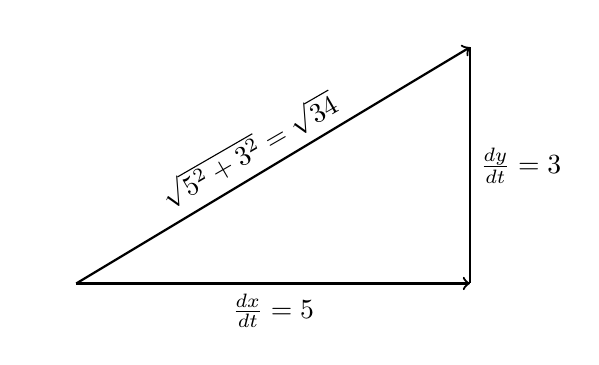
\begin{tikzpicture}[]



\draw[->,thick] (0,0) -- (5,0) node[above] {};
\draw[- ,thick] (5,0) -- (5,3) node[above] {};
\draw[->,thick] (0,0) -- (5,3) node[above] {};
\draw[-,thick] (-0.5,-.5) node[above] {};
\draw[-,thick] (2.5,0) node[below] {$\frac{dx}{dt}=5$};
\draw[-,thick] (5,1.5) node[right] {$\frac{dy}{dt}=3$};
\draw[-,thick] (1,1) node[right, rotate = 30] {$\sqrt{5^2+3^2}=\sqrt{34}$};

\end{tikzpicture}


	
\end{document}
